\section{Bug Reporting in Open Source Projects}


%The problem is real, i.e., there are repos that have more BRs than they can manage. How many BRs arrive at the most popular repos (is the traffic bursty)? how many lack OB/EB/S2R from these?
The overall trend in software development in recent years is towards increased
speed of development and delivery. There are nowadays numerous projects on popular
public software collaboration platforms like GitHub that have large development
teams and user communities. Many of these projects experience significant
bug reporting traffic. Figure~\ref{fig:repo_activity} shows the issue creation
frequency for a selection of 10 GitHub repositories that are currently active
with a high numbers of commits???.

\begin{figure}[t]
\centering
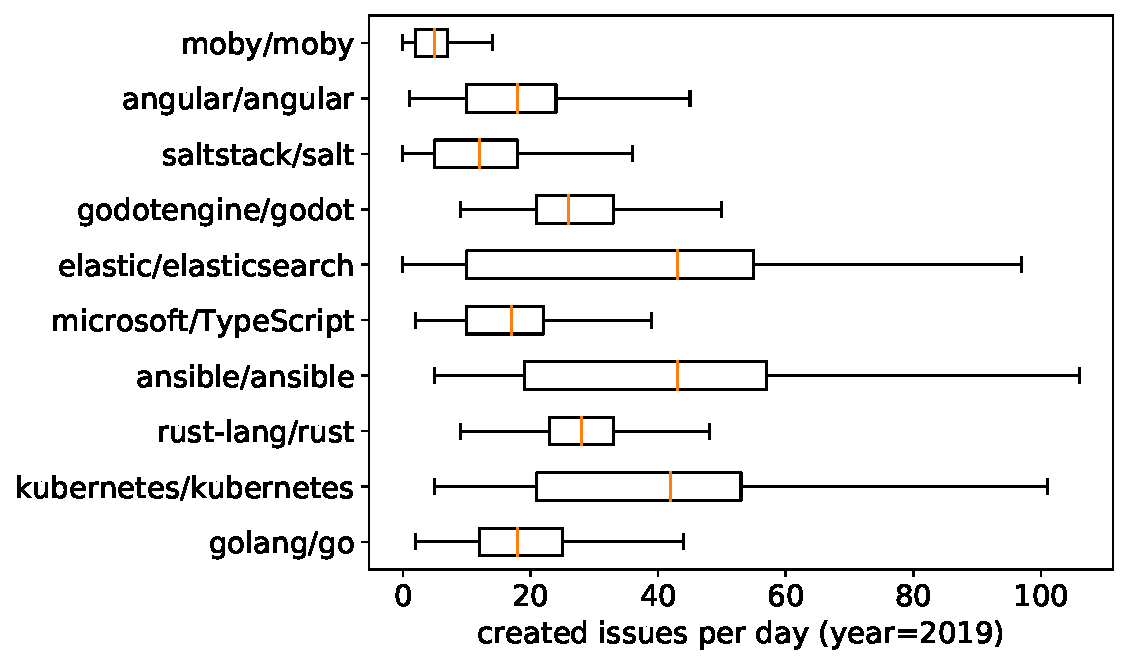
\includegraphics[width=0.99\linewidth]{figures/popular_repos.pdf}
\caption{...}
\label{fig:repo_activity}
\end{figure}



The preconditions are present, i.e., there are a lot of follow-up questions on GitHub






Motivate the value of the answer as a way of ranking
